\section{Why interpretability?}
Modern machine learning models based on deep neural networks are achieving remarkable performance in many fields. In comparison with classic machine learning technologies like decision trees, it is much harder to explain how these neural networks came to their conclusions, because they use thousands to millions of training parameters.

Especially in the medical imaging field, it is very important that algorithms not only generate a correct diagnosis when training the algorithm, but also shows that its using the same cues in images as do trained physicians. These cues are found and verified in scientific studies, and therefore are well understood and proved to be correct. A wrong diagnosis generated by a neural network reduce the confidence of physic ans using the technology or even be life threatening when used without professional supervision.

\section{Methods for classification}
In recent years, many methods for the interpretability of deep (convolutional) neural networks have been proposed, e.g. LIME \cite{ribeiro2016should}, RISE \cite{Petsiuk2018rise}, Grad-CAM \cite{selvaraju2017grad} or DeepLIFT \cite{shrikumar2017learning}.

\begin{figure}[h]
\centering
\caption{Examples of some interpretability methods for image classification \cite{visualattribution}}
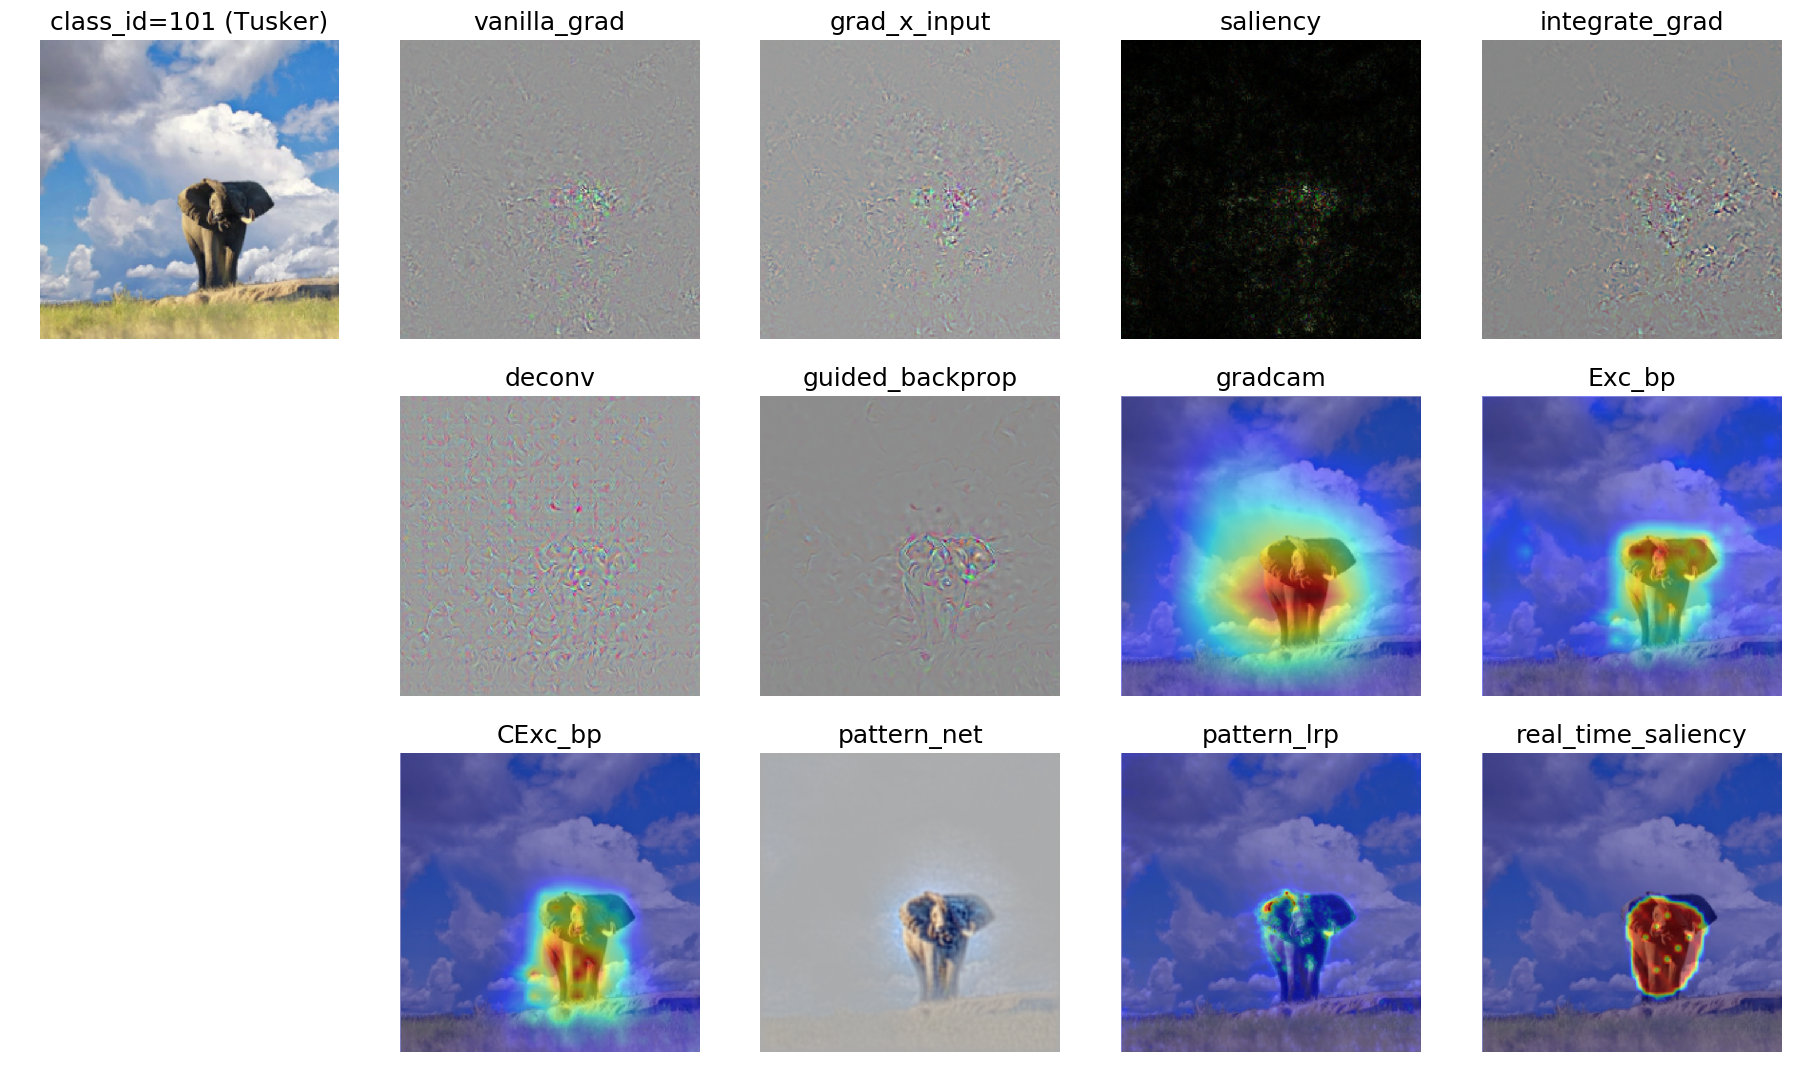
\includegraphics[width=14cm]{images/tusker_saliency.png}
\end{figure}

These methods focus on providing explanations and interpretability of classification problems for datasets like ImageNet \cite{imagenet_cvpr09} or MNIST \cite{lecun-mnisthandwrittendigit-2010}. Classification means that an algorithm can tell what is displayed on an image, e.g. if and what kind of disease is visible on a x-ray or MRI scan.

\section{Image segmentation}
Image segmentation is different from classification in the way that the algoriths do not detect what is visible on a picture, but instead mark a region (the segment) in an image where it thinks something is visible. For example for self driving cars, it is important to know where the car or pedestrian in front of the car is. 

In the medical imaging field, one applications is the segmentation of tumors in MRI scans.

\section{Interpretability on image segmentation}
TODO => does not really exist yet

\section{Source Code}
The source code of the thesis is available on GitHub:
\begin{itemize}
    \item Thesis source code (mostly jupyter notebooks): \url{https://github.com/andef4/thesis-code}
    \item Python library source code: \url{https://github.com/andef4/interpret-segmentation}
    \item Latex source for this document: \url{https://github.com/andef4/interpret-segmentation}
\end{itemize}

All source code is licensed under the permissive MIT license.